\documentclass{beamer}
\usetheme{metropolis}
\usepackage{graphicx}
\usepackage{amsmath}
\usepackage{tcolorbox}
\title{Elementary Statistics: Math 080}
\author{Jordan Hanson}
\institute{Whittier College Department of Physics and Astronomy}

\begin{document}
\maketitle

\begin{frame}{Course Introduction}
\begin{enumerate}
\item \textit{\textbf{\alert{What is statistical analysis?}}}
\item Math 080: Elementary Statistics
\item Read the syllabus for a roadmap
\item This is an online summer course that meets each day.
\item \textbf{Data science project and presentation}
\item Textbook: \url{https://openstax.org/details/books/introductory-statistics}
\item Download and install Excel, or LibreOffice Calc
\end{enumerate}
\end{frame}

\begin{frame}{Lecture format, with modifications}
\begin{itemize}
\item Warm-up exercise, and solution
\item Lecture via Whiteboard and slides
\item Interactive questions or polls
\item Laboratory activity (asynchronous)
\item Asynchronous content
\begin{enumerate}
\item Homework clues
\item Example problems
\item Special topics
\end{enumerate}
\end{itemize}
\end{frame}

\begin{frame}{Unit 0 Outline}
\begin{enumerate}
\item Topics from Chapter 1: 1.1, 1.2, 1.3
\begin{itemize}
\item What is a statistic?
\item Probability examples
\item Data and sampling
\end{itemize}
\item Topics from Chapter 2: 2.1 - 2.4, 2.5 - 2.8
\begin{itemize}
\item Data visualization
\item Location of the data in numerical space
\end{itemize}
\item Topics from Chapter 3: 3.1, 3.2, 3.3
\begin{itemize}
\item Two rules of probability
\end{itemize}
\end{enumerate}
\end{frame}

\section{Topics from Chapter 1}

\begin{frame}{What is statistical analysis?}
By tradition, we begin with Mark Twain.
\begin{figure}
\centering
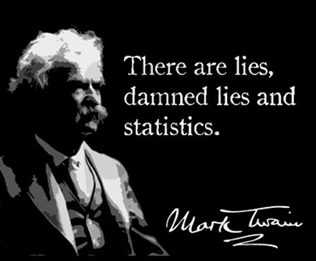
\includegraphics[width=0.6\textwidth]{figures/twain.png}
\caption{A famous quote from Mark Twain.}
\end{figure}
\end{frame}

\begin{frame}{Warm-up exercises}
\small
\textbf{COVID-19 data.}  In a March 2020 article in the magazine \texttt{wired.com}, Ferris Jabr points out that people were drawing comparisons between the influenza pandemic of 1918 and SARS-Cov-2 (COVID-19).  The \alert{case fatality rate}, or CFR, is the percentage of people who contract the disease that perish from it.  In the 1918 outbreak, it is usually stated that there were approximately 500 million infections, 50-100 million fatalities, and an overall CFR of 2.5\%.  What is interesting is that the coronavirus seems to have a CFR (averaged over age) of $\approx 3$ \%, making it ... \textit{higher}. \\ \vspace{0.5 cm}
Question 1: The above paragraph listed four pieces of data.  What are they? \\
\end{frame}

\begin{frame}{Warm-up exercises}
\small
\textbf{COVID-19 data.}  In a March 2020 article in the magazine \texttt{wired.com}, Ferris Jabr points out that people were drawing comparisons between the influenza pandemic of 1918 and SARS-Cov-2 (COVID-19).  The \alert{case fatality rate}, or CFR, is the percentage of people who contract the disease that perish from it.  In the 1918 outbreak, it is usually stated that there were approximately 500 million infections, 50-100 million fatalities, and an overall CFR of 2.5\%.  What is interesting is that the coronavirus seems to have a CFR (averaged over age) of $\approx 3$ \%, making it ... \textit{higher}. \\ \vspace{0.5 cm}
Question 2: Which number, if any, seems to have a problem?
\begin{itemize}
\item A: The total number of infections in 1918
\item B: The total number of deaths in 1918
\item C: The 1918 influenza CFR
\item D: The 2020 coronavirus CFR
\end{itemize}
\end{frame}

\begin{frame}{Warm-up exercises}
\small
\textbf{COVID-19 data.}  In a March 2020 article in the magazine \texttt{wired.com}, Ferris Jabr points out that people were drawing comparisons between the influenza pandemic of 1918 and SARS-Cov-2 (COVID-19).  The \alert{case fatality rate}, or CFR, is the percentage of people who contract the disease that perish from it.  In the 1918 outbreak, it is usually stated that there were approximately 500 million infections, 50-100 million fatalities, and an overall CFR of 2.5\%.  What is interesting is that the coronavirus seems to have a CFR (averaged over age) of $\approx 3$ \%, making it ... \textit{higher}. \\ \vspace{0.5 cm}
Question 3: From the rest of the data in the paragraph, estimate the proper CFR of the 1918 influenza.  Compare this number with the CFR of the 2020 coronavirus.
\end{frame}

\begin{frame}{Topics from Chapter 1}
\small
\textit{Vocabulary}:
\begin{enumerate}
\item \textbf{Probability}: The extend to which something is \textit{likely} to occur, measured by the ratio of favorable cases to the whole number of cases possible.
\item \textbf{Population}: The total collection of people, objects, or cases under investigation.
\item \textbf{Sample}: A subset of the population for which statistical data is collected.
\item \textbf{Statistic}: \textit{A statistic} is a number that represents a property of the sample.  For example: the CFR of a \textit{sample} of 2,500 coronavirus patients.
\item \textbf{Parameter}: Statistic measured from the \textit{entire} population.  A statistic attempts to reveal knowledge of a parameter.
\end{enumerate}
\end{frame}

\begin{frame}{Topics from Chapter 1}
\small
\textit{Vocabulary}:
\begin{enumerate}
\item \textbf{Representative sample}: a sample that captures all of the properties of a population. Counter-example: psychological studies using undergraduate subjects.
\item \textbf{Variable}: A property of each member of the population that can be determined, either quantitative or categorical. \textbf{Data} are the actual values.
\end{enumerate}
\end{frame}

\begin{frame}{Topics from Chapter 1}
\begin{tcolorbox}[colback=orange!10,colframe=orange!100,title=Mean: Definition 1]
Let X represent a \textit{variable} of a \textit{population}, and $x_i$ represent the actual value of the i-th member of a statistical \textit{sample} of that \textit{population}.  The arithmetic mean $\bar{x}$ of the \textit{sample} for that property is
\begin{equation}
\bar{x} = \frac{1}{N}\sum_i^{N} x_i
\end{equation}
\end{tcolorbox}
The mean of the variable X is the number $\bar{x}$ from the sample.
\end{frame}

\begin{frame}{Topics from Chapter 1}
Example 1: What's the average number of siblings in our community?
\begin{enumerate}
\item What is the population?
\item What is the sample?  (Our class).
\item What is the variable?
\item What are the data?
\end{enumerate}
\textbf{Write in the chat area the number of siblings in your family, including yourself.}
\end{frame}

\begin{frame}{Topics from Chapter 1}
Example 2: How many languages do you speak?
\begin{enumerate}
\item What is the population?
\item What is the sample?  (Our class).
\item What is the variable?
\item What are the data?
\end{enumerate}
\textbf{Write in the chat area the number of languages that you can speak.}
\end{frame}

\begin{frame}{Topics from Chapter 1}
\small
\textit{Vocabulary}:
\begin{enumerate}
\item \textbf{Proportion}: The total number of subjects in the sample that share a property, divided by the total number of subjects in the sample.
\item \textbf{Qualitative data}: Sometimes called categorical data, refers to non-numerical properties of subjects in sample (e.g. place of birth).
\item \textbf{Quantitative data}: Numerical values of variables for each subject in a sample (e.g. age).
\begin{itemize}
\item Continuous quantitative data: average hours of sleep per night
\item Discrete quantitative data: average number of siblings
\end{itemize}
\end{enumerate}
\end{frame}

\begin{frame}{Topics from Chapter 1}
Example 1: What fraction of Whittier College students live on campus?
\begin{enumerate}
\item What is the population?
\item What is the sample?  (Our class).
\item What is the variable?
\item What are the data?
\end{enumerate}
\textbf{Write in the chat area the number 1 if you live on-campus, and the number 0 if you live off-campus or with your family.} \\ \vspace{0.5cm}
Whittier College Factbook: 46.3\% of undergraduates live on-campus.
\end{frame}

\begin{frame}{Topics from Chapter 1}
Example 2: What is the proportion of students to instructors here?  (What is the student to faculty ratio of Whittier College)?
\begin{enumerate}
\item What is the population?
\item What is the sample?  (Our class).
\item What is the variable?
\item What are the data?
\end{enumerate}
\textbf{Let's sum the students here, and then there is me.} \\ \vspace{0.5cm}
Whittier College Factbook: average student to faculty ratio: 11
\end{frame}

\begin{frame}{Topics from Chapter 1}
\small
Example 3: You go to the supermarket and purchase three cans of soup:
\begin{itemize}
\item 19 ounces tomato bisque
\item 14.1 ounces lentil
\item 19 ounces Italian wedding
\end{itemize}
...and two desserts:
\begin{itemize}
\item 16 ounces pistachio ice cream
\item 32 ounces chocolate chip cookies
\end{itemize}
\textbf{Create three data sets: one quantitative discrete, one quantitative continuous, and one categorical.}
\end{frame}

\section{Laboratory Activity}

\begin{frame}{Laboratory Activity}
Go to the following link and watch the interesting TED talk by Steven Levitt from 2005 about driving safety. \\ \vspace{1cm}
\url{https://www.ted.com/talks/steven_levitt_surprising_stats_about_child_carseats?utm_campaign=tedspread&utm_medium=referral&utm_source=tedcomshare} \\ \vspace{1cm}
Answer the questions on the form entitled \alert{Laboratory Exercise 1} on Moodle for this week, and submit them via email: jhanson2@whittier.edu. (This is part of your warm-ups grade...see syllabus).
\end{frame}

\section{Interactive Questions}

\begin{frame}{Interactive Questions}
Almost always, we will give multiple-choice questions with answers A-D.  If you are lost, or need extra explanation, or just feel we are going to fast, select the letter E.  E stands for WAT...
\begin{figure}
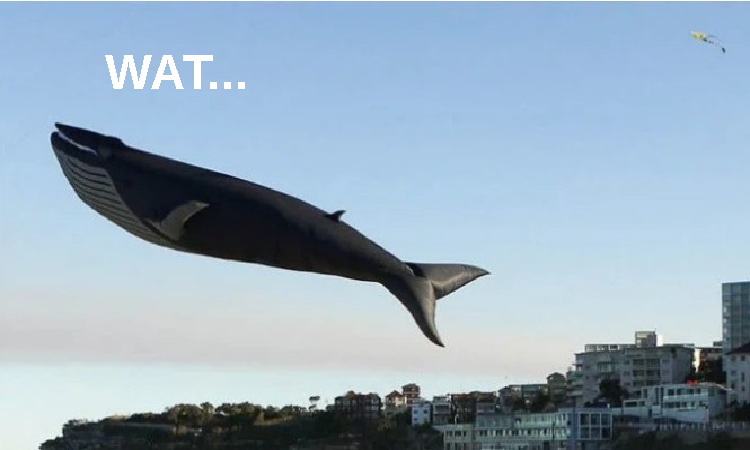
\includegraphics[width=0.5\textwidth]{figures/wat.pdf}
\end{figure}
After 1 round, we examine the \textit{answer distribution}, and if 70\% get it right, we move on.  Otherwise, we discuss via chat with each other, explaining why we picked our answer.  Then we have round 2.  Remember to hit E if you are confused.
\end{frame}

\begin{frame}{Interactive Questions}
To battle the pandemic, backup health care workers were called in to work in hospitals A, B, and C.  Hospital A began with 50, hospital B began with 40, and hospital C began with 60.  Hospital A received an additional 10, B received an additional 25, and C received an additional 5.  What is the average number of workers at hospitals in this sample (A, B, and C)?
\begin{itemize}
\item A: 53
\item B: 63
\item C: 42
\item D: 32
\end{itemize}
\end{frame}

\begin{frame}{Interactive Questions}
Suppose a sample of students record the duration of their sleep each night for a week, and gather the data at the end.  What kind of data is this?
\begin{itemize}
\item A: Quantitative discrete
\item B: Qualitative or categorical
\item C: Quantitative continuous
\item D: Variable
\end{itemize}
\end{frame}

\begin{frame}{Interactive Questions}
\begin{figure}
\centering
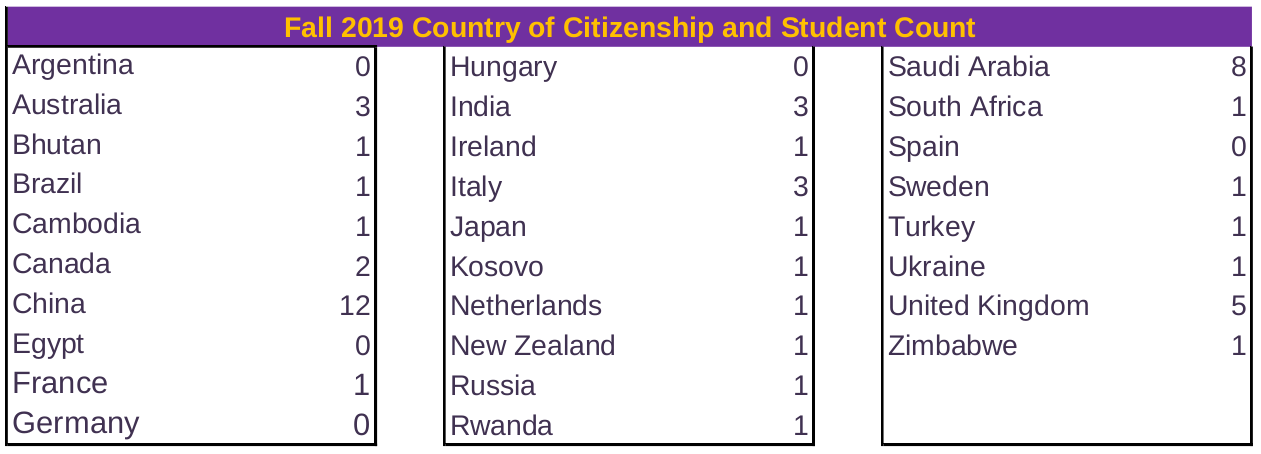
\includegraphics[width=0.85\textwidth]{figures/map.png}
\end{figure}
What kind of data is represented in the population above? (There may be more than one answer).
\begin{itemize}
\item A: Quantitative discrete
\item B: Qualitative or categorical
\item C: Quantitative continuous
\item D: Variable
\end{itemize}
\end{frame}

\begin{frame}{Interactive Questions}
\begin{figure}
\centering
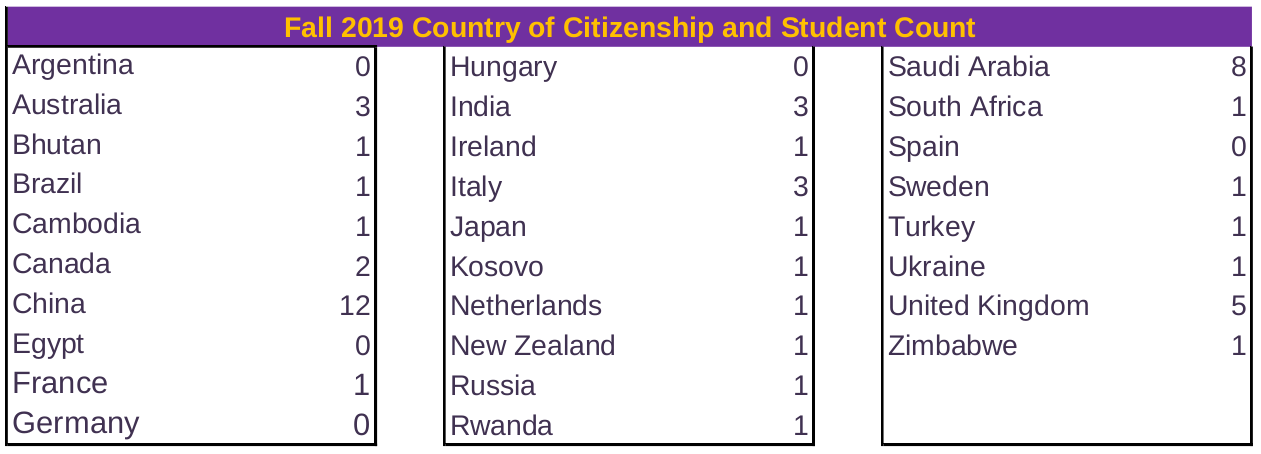
\includegraphics[width=0.85\textwidth]{figures/map.png}
\end{figure}
The total number of international students is 52 in the above table.  What proportion of international students are from China?
\begin{itemize}
\item A: 12
\item B: 12\%
\item C: 23
\item D: 23\%
\end{itemize}
\end{frame}

\begin{frame}{Interactive Questions}
\begin{figure}
\centering
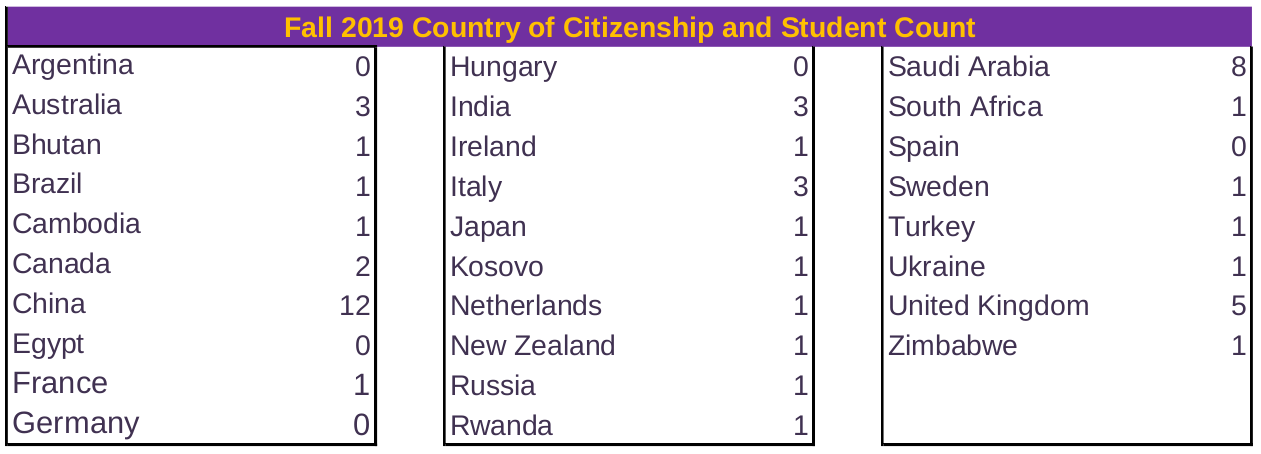
\includegraphics[width=0.85\textwidth]{figures/map.png}
\end{figure}
The total number of international students is 52 in the above table.  What proportion of international students are from Europe?
\begin{itemize}
\item A: 15\%
\item B: 23\%
\item C: 50\%
\item D: 12
\end{itemize}
\end{frame}

\section{Other forms of Qualitative Data, Sampling}

\begin{frame}{Other forms of Qualitative Data}
\begin{enumerate}
\item Types of categories
\item Overlapping and non-overlapping categories, missing data
\item Activity on Pareto charts
\item Sampling strategies
\end{enumerate}
\end{frame}

\begin{frame}{Qualitative Data}
\begin{figure}
\centering
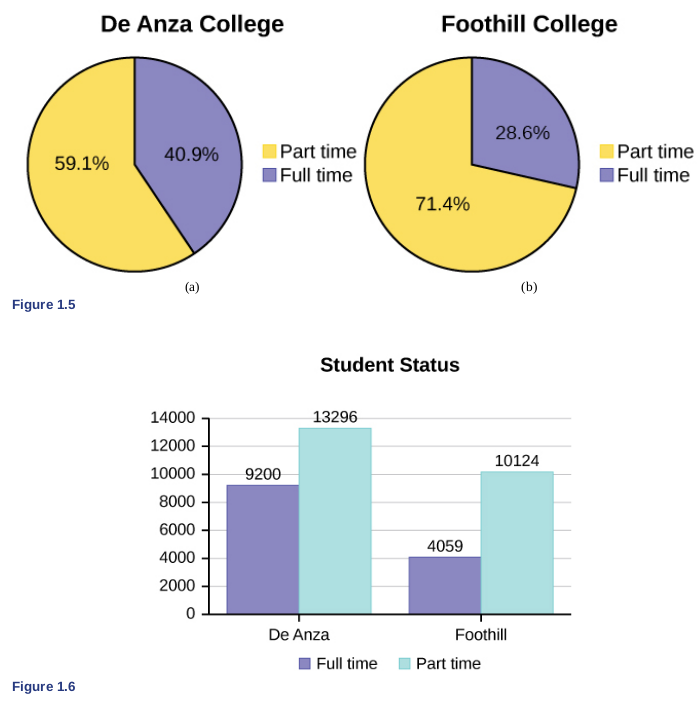
\includegraphics[width=0.6\textwidth]{figures/qualitativeData.png}
\caption{\label{fig:qual} Two types of qualitative data representation.}
\end{figure}
\end{frame}

\begin{frame}{Qualitative Data}
\begin{enumerate}
\item \textbf{Mulitple categories}: Categories can overlap, so when calculating proportions, the percentatge can sum to greater than 100 percent.
\begin{itemize}
\item Proportion of first-year students who are female: 56\%
\item Proportion of students who are male: 44\%
\item Proportion of students who do not live on campus: 46\%
\end{itemize}
\item \textbf{Missing categories}: Categories do not always capture every feature of a population.
\begin{figure}
\centering
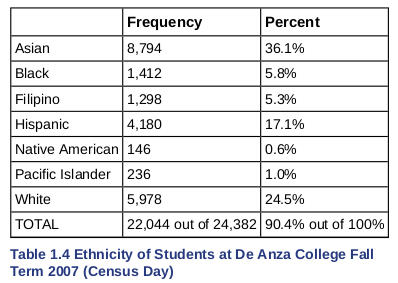
\includegraphics[width=5cm]{figures/race.png}
\end{figure}
\end{enumerate}
\end{frame}

\begin{frame}{Qualitative Data}
\begin{figure}
\centering
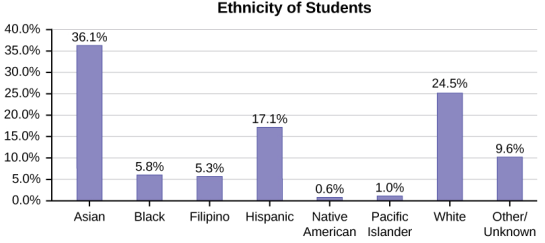
\includegraphics[width=6cm]{figures/race2.png}
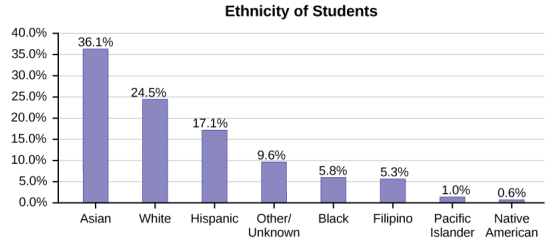
\includegraphics[width=6cm]{figures/race3.png}
\caption{\label{fig:pareto} A Pareto chart is a bar graph that is ordered greatest to least.  This can sometimes illuminate an effect that wasn't obvious.}
\end{figure}
\end{frame}

\begin{frame}{Qualitative Data}
\small
\begin{columns}[T]
\begin{column}{0.55\textwidth}
Let's create a Pareto chart from the Whittier College factbook.
\begin{figure}
\centering
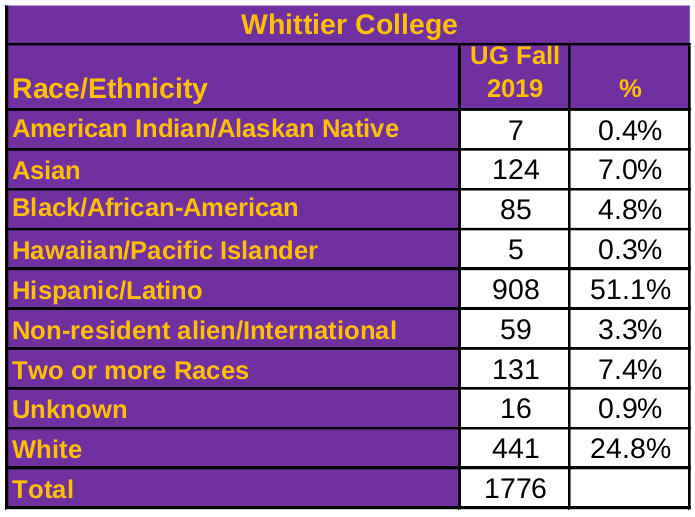
\includegraphics[width=4cm]{figures/race4.png}
\caption{\label{fig:pareto2} The demographic breakdown of Whittier College undergraduate self-reported ethnicity data from 2019-20.}
\end{figure}
\end{column}
\begin{column}{0.45\textwidth}
\begin{itemize}
\item Open your copy of Excel, or LibreOffice Calc
\item Make one column heading entitled \textbf{ETH}
\item Make one column heading entitled \textbf{N}
\item Copy the data in Fig. \ref{fig:pareto2} into your columns
\end{itemize}
\end{column}
\end{columns}
\end{frame}

\begin{frame}{Qualitative Data}
\small
\begin{columns}[T]
\begin{column}{0.5\textwidth}
Let's create a Pareto chart from the Whittier College factbook.
\begin{figure}
\centering
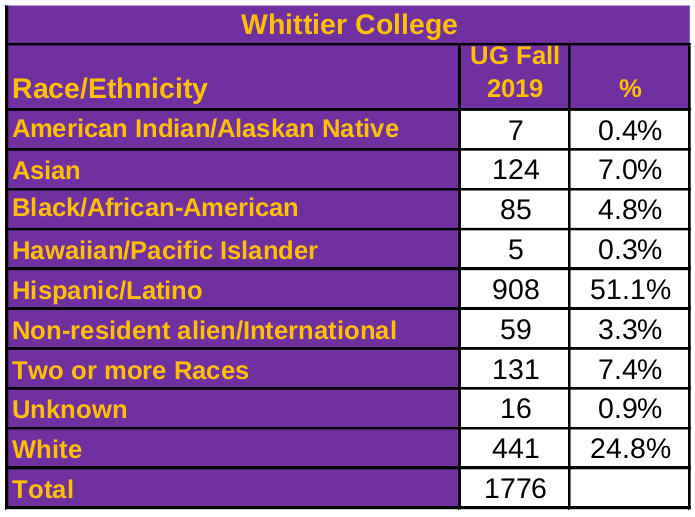
\includegraphics[width=4cm]{figures/race4.png}
\caption{\label{fig:pareto3} The demographic breakdown of Whittier College undergraduate self-reported ethnicity data from 2019-20.}
\end{figure}
\end{column}
\begin{column}{0.5\textwidth}
\begin{itemize}
\item Sort the data according to \textbf{N}
\item Click the menu ``Insert,'' and insert a bar chart
\end{itemize}
\begin{figure}
\centering
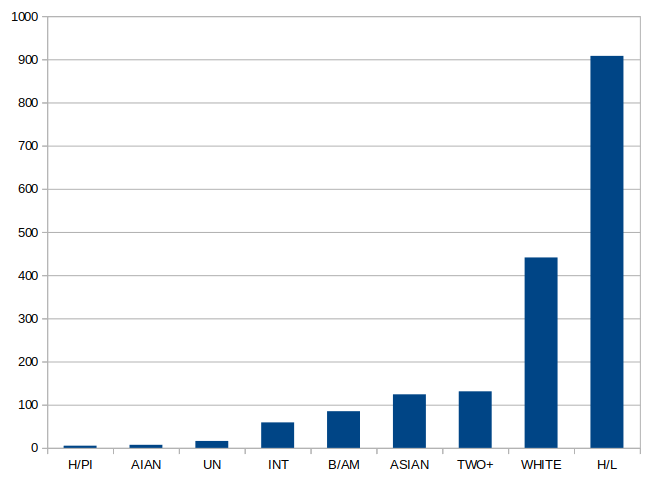
\includegraphics[width=5cm]{figures/race5.png}
\caption{A Pareto chart of Whittier College ethnicity data.  The sample is the UG as of Fall 2019.}
\end{figure}
\end{column}
\end{columns}
\end{frame}

\begin{frame}{Sampling Strategies}
\alert{Sampling Strategies:}
\begin{itemize}
\item Simple random ... how to generate random numbers? (Good project).
\item Stratified sampling: pre-defined groups, choose proportionately at random from those groups (choosing at random from Depts.)
\item Cluster sampling: pre-defined groups, but choose \textit{the groups themselves} at random (choose random Depts.)
\item Systematic sampling: select every n-th subject in the population to form the sample (assume some ordering, could be random)
\end{itemize}
\end{frame}

\begin{frame}{Sampling Strategies}
\textbf{Cool example on random sampling.}  How can you measure the number of fish in a pond?  Catch all the fish?  No way!  Use simple random sampling.
\begin{enumerate}
\item Catch $n$ fish, and mark them.
\item Return one day later, and catch $n$ fish again.
\item Assume the sample of fish is \textit{simple random}.  Why is this a good or bad assumption?
\item Measure the number $m$ of marked fish, caught the second day.
\item The \textit{proportion of total fish that are marked} is $p = m/n$.
\item But, $p = n/N$, where $N$ is the total...
\item $N = n/p = n^2/m$. \vspace{0.5cm} \footnote{Proceed to Hawai'i to tag great white sharks...}
\end{enumerate}
\end{frame}

\begin{frame}{Sampling Strategies}
\textbf{Cool example on random sampling.}  How can you measure the number of fish in a pond?  Catch all the fish?  No way!  Use simple random sampling.
\begin{enumerate}
\item With replacement ... keeps the population unchanged, randomness preserved.
\item Without replacement ... changes the population by 1 with each choice.  Often more convenient and does not matter as long as the sample size is ``large enough.''
\end{enumerate}
\end{frame}

\begin{frame}{Sampling Strategies}
\alert{Systematic sampling}, special case: waveform data, time-series data.  Systmatic trends cannot be observed by data sampled insufficiently systematically.
\begin{figure}
\centering
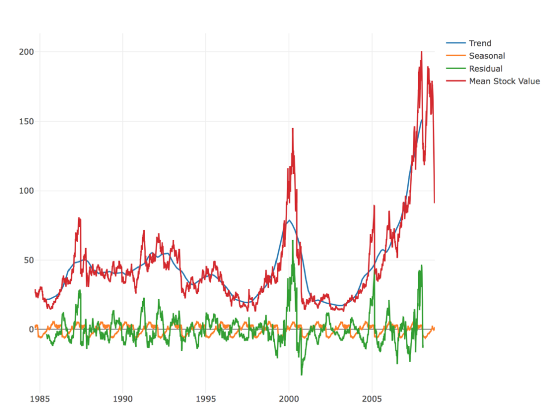
\includegraphics[width=0.6\textwidth]{figures/stock.png}
\caption{Example of stock price data.}
\end{figure}
\end{frame}

\section{Laboratory Activity}

\begin{frame}
Go to the following link to watch a TED talk by the one, the only, Malcom Gladwell: \\ \vspace{1cm}
\url{https://www.ted.com/talks/malcolm_gladwell_choice_happiness_and_spaghetti_sauce?utm_campaign=tedspread&utm_medium=referral&utm_source=tedcomshare} \\ \vspace{1cm}
Answer the questions on the form entitled \alert{Laboratory Exercise 2} on Moodle for this week, and submit them via Moodle.
\end{frame}

\section{Interactive Questions}

\begin{frame}{Interactive Questions}
The instructor takes her sample by gathering data on five randomly selected students from each Lake Tahoe Community College math class. The type of sampling she used is
\begin{itemize}
\item A: Cluster sampling
\item B: Stratified sampling
\item C: Simple random sampling
\item D: Convenience sampling
\end{itemize}
\end{frame}

\begin{frame}{Interactive Questions}
A study was done to determine the age, number of times per week, and the duration (amount of time) of residents using
a local park in San Jose. The first house in the neighborhood around the park was selected randomly and then every eighth
house in the neighborhood around the park was interviewed. The sampling method was:
\begin{itemize}
\item A: Simple random
\item B: Systematic
\item C: Stratified
\item D: Cluster
\end{itemize}
\end{frame}

\begin{frame}{Interactive Questions}
Suppose you are working at a shoe company, and you sample the preferences of 5,000 previous customers to inform a new shoe design.  If the response rate is 20 percent, and 300 responses indicated customers prefered leather to rubber insteps, what proportion of the random sample does this represent?
\begin{itemize}
\item 30 percent
\item 20 percent
\item 20 percent
\item 10 percent
\end{itemize}

\end{frame}

\section{Frequency, Relative Frequency}

\begin{frame}{Frequency, Relative Frequency}
\alert{How frequently do data values occur in the sample?}
An activity to demonstrate the concept of frequency. \\ \vspace{0.5cm}
\url{https://phet.colorado.edu/en/simulation/plinko-probability}
\end{frame}

\begin{frame}{Frequency, Relative Frequency}
\begin{enumerate}
\item Begin with the Intro tab to this PhET simulation.
\item Use the controls at upper right to drop balls through the Plinko system.
\item Notice how they have \textit{more or less} an equal chance of bouncing to the left or right at each level.
\item This behavior of being equally likely leads to a variation in the frequency with which objects land in the areas below.
\end{enumerate}
\end{frame}

\begin{frame}{Frequency, Relative Frequency}
\small
\begin{enumerate}
\item Now click the Lab tab at the bottom center of the screen.
\item Use the controls at right to increase the rows to 26.
\item Leave the ``binary probability'' set to 0.5, meaning 50\% chance left, 50\% chance right, at each interaction.
\item We have encountered how to calculate the mean $\bar{x}$ from a data sample.  The mean position of all the balls is given at bottom right.
\item Use the play button at top right to drop 1,000 balls to form a data sample of positions at the bottom.
\item When you reach 1000, copy the \textit{bins} (0, ... , 26) and the \textit{frequencies} (the data in the bins) into Excel or LibreOffice Calc.  Put the bin numbers in column A, and the frequencies the adjacent column B.
\end{enumerate}
\end{frame}

\begin{frame}[fragile]{Frequency, Relative Frequency}
\small
\begin{enumerate}
\item Suppose you want to sum the frequencies.  In a cell below the column of frequency data, type
\begin{verbatim}
=SUM(B1:B27)
\end{verbatim}
and hit enter.  This assumes that your data is in column B, in cells 1 through 27.
\item This should be the $N$ value given by the PhET simulation (close to 1000).
\item In column C, cell 1, type
\begin{verbatim}
=B1/N
\end{verbatim}
Instead of $N$, though, type the result for $N$ found above.
\item Click on cell C1, and drag the little black square at the bottom right of the cell down until you reach C27 (repeats the calculation).
\end{enumerate}
\end{frame}

\begin{frame}[fragile]{Frequency, Relative Frequency}
\small
\begin{enumerate}
\item Column C data are known as \textit{relative frequencies.}  They represent the probability of discovering a data result with the bin value.
\item If you use the SUM function to sum the relative frequencies, what result is obtained?
\item What about a ``running total'' of relative frequencies, to keep track of how quickly we approach 100\% of the data?  In cell D1, type
\begin{verbatim}
=C1
\end{verbatim} 
and in cell D2, type
\begin{verbatim}
=C2+D1
\end{verbatim}
Click and drag to repeat the calculation until you reach the last cell.  This trick adds the new C value to the running total. Create a plot of bin value versus column D.
\item Column D is the \textit{cumulative frequency} of the data sample.
\end{enumerate}
\end{frame}

\begin{frame}{Topics from Chapter 1}
\begin{tcolorbox}[colback=orange!10,colframe=orange!100,title=Mean: Definition 2]
Let X represent a statistical variable, and $x_i$ represent the data values.  Suppose there are $n_i$ instances of $x_i$, with only $M$ unique values.  The $n_i$ are the \textit{frequencies}, and we can write
\begin{equation}
\bar{x} = \frac{1}{N}\sum_i^{M} n_i x_i
\end{equation}
Moving the $1/N$ inside the sum, we see that
\begin{equation}
\bar{x} = \sum_i^{M} \left(\frac{n_i}{N}\right) x_i = \sum_i^{M} f_i x_i
\end{equation}
\end{tcolorbox}
The fraction $f_i = n_i/N$ are the relative frequencies.  (Professor: do an example).
\end{frame}

\section{Conclusion}

\begin{frame}{Unit 0 Outline}
\begin{enumerate}
\item Topics from Chapter 1: 1.1, 1.2, 1.3
\begin{itemize}
\item What is a statistic?
\item Probability examples
\item Data and sampling
\end{itemize}
\item Topics from Chapter 2: 2.1 - 2.4, 2.5 - 2.8
\begin{itemize}
\item Data visualization
\item Location of the data in numerical space
\end{itemize}
\item Topics from Chapter 3: 3.1, 3.2, 3.3
\begin{itemize}
\item Two rules of probability
\end{itemize}
\end{enumerate}
\end{frame}

\end{document}
